\subsection{Monitoraggio e Intervento}
% descrizione implementazione Neural ODE per controller automatico
% descrizione funzione di controllo e implementazione con modello
% descrizione funzione di controllo del controllo 
% varie assunzioni 

\subsubsection{SciML.ai}

L'utilizzo della suite \textbf{SciML.ai} e' stato fatto per l'integrazione
di un modello di Machine Learning in un sistema di monitoraggio e possibilmente di 
intervento. Applicare un algoritmo di ML per predire l'andamento di un sistema non lineare dinamico 
senza avere una grande base di dati puo' risultare problematico e i risultati possono risultare 
poco affidabili. Lo sviluppo di tecniche che congiungono la modellazione puramente matematica
alla flessibilita' delle reti neurali ha permesso di sviluppare approcci \emph{data-driven domain-specific} 
\cite{rackauckas2020universal} \cite{Kim_2021} \cite{dandekar2022bayesian} \cite{chen2019neural}
che permettono di ottenere risultati affidabili pur avendo una base di dati scarsa.

\subsubsection*{Addestramento}
Viene definito il sistema di ODE che fara' da base per l'addestramento della \textbf{Neural ODE} \cite{chen2019neural}
e successivamente viene definita la rete neurale tramite la suite \textbf{Lux.jl} \cite{pal2023lux}.
Questo permette di definire facilmente e velocemente una rete neurale che verra' usata 
in coppia con il sistema di ODE per ottenere il meglio da entrambi, andando a definire 
quello che viene chiamato \textbf{Scientific Machine Learning}.

\begin{figure}[!hb]
	\centering
	\begin{subfigure}[b]{0.45\textwidth}
		\centering
		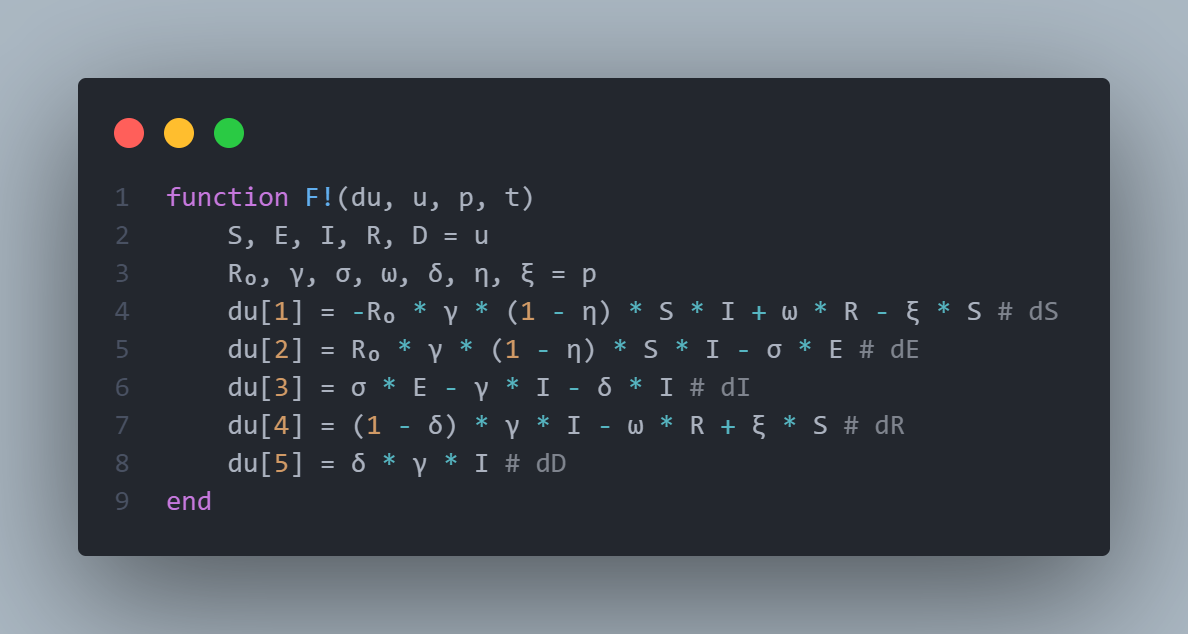
\includegraphics[width=\textwidth]{img/seir_function.png}
		\caption{Definizione del sistema di ODE per l'addestramento della rete neurale}
		\label{fig:seir_function}
	\end{subfigure}
	\hfill
	\begin{subfigure}[b]{0.45\textwidth}
		\centering
		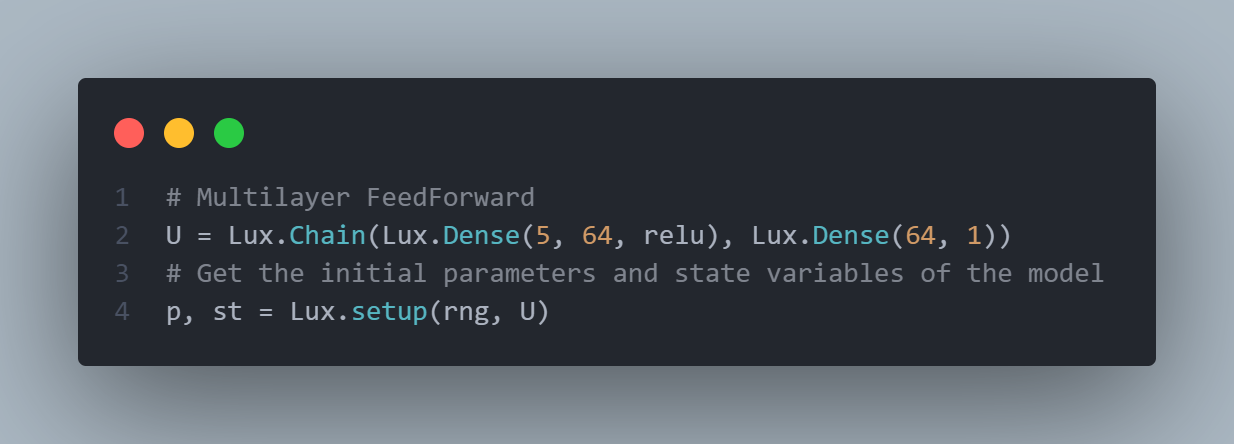
\includegraphics[width=\textwidth]{img/neural_ode.png}
		\caption{Definizione della rete neurale}
		\label{fig:neural_ode}
	\end{subfigure}
\end{figure}

Dopo aver definito queste due funzioni, vengono definite le regole di predizione
per l'addestramento e le regole della funzione di loss. La funzione di loss viene definita 
come la loss L2 ovvero un \textbf{Mean Squared Error (MSE)} o \textbf{Errore Quadratico Medio}
\cite{wiki:Mean_squared_error}.

\begin{figure}[!hb]
	\centering
	\begin{subfigure}[b]{0.45\textwidth}
		\centering
		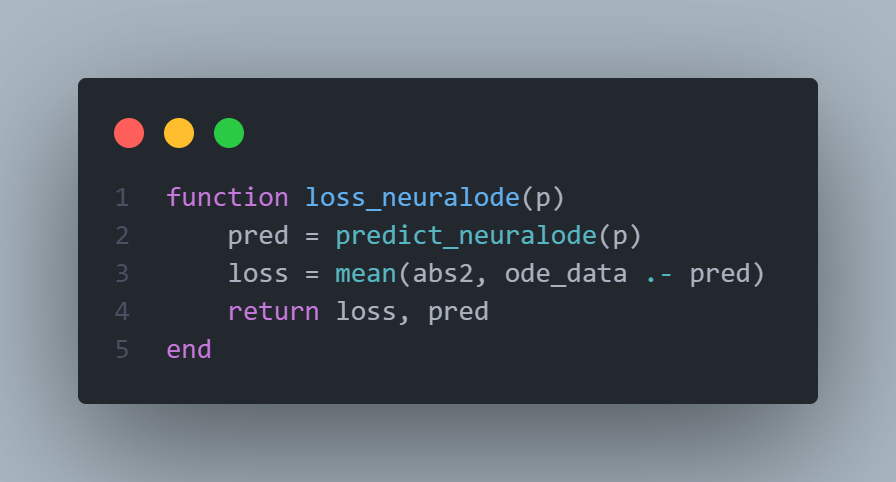
\includegraphics[width=\textwidth]{img/loss.png}
		\caption{Definizione della funzione di Loss}
		\label{fig:loss_function}
	\end{subfigure}
	\hfill
	\begin{subfigure}[b]{0.45\textwidth}
		\centering
		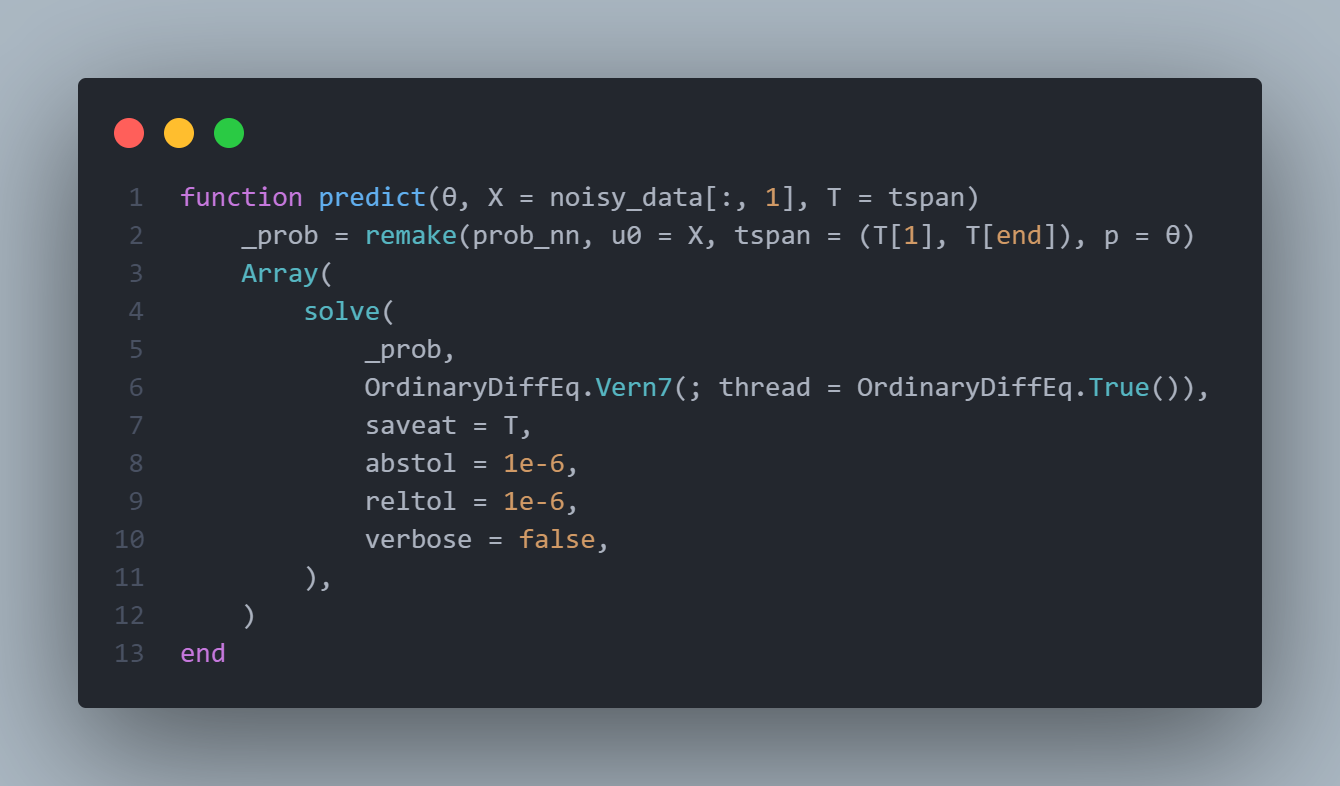
\includegraphics[width=\textwidth]{img/predict_function.png}
		\caption{Definizione del loop di addestramento}
		\label{fig:predict_function}
	\end{subfigure}
\end{figure}

Utilizzando poi le regole di ottimizzazione offerte dal framework \textbf{Optimization.jl} \cite{vaibhav_kumar_dixit_2023_7738525}
e' possibile definire una struttura di controllo tramite la creazione di un 
\textbf{OptimizationProblem} e una \textbf{OptimizationFunction} e la scelta di un 
algoritmo di ottimizzazione, generalmente lasciato automatico, e' possibile addestrare
la propria \emph{Neural ODE}.

\begin{minipage}{\linewidth}
	\centering
	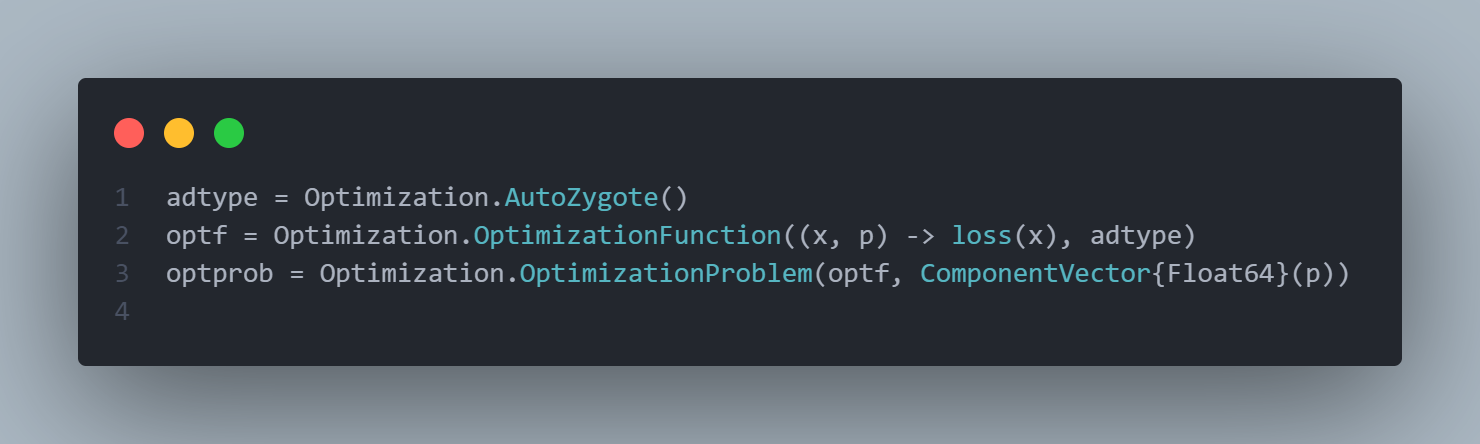
\includegraphics[width=\textwidth]{img/optimization_functions.png}
	\captionof{figure}{Definizione delle funzioni di ottimizzazione}
	\label{fig:optimization_function}
\end{minipage}

Per ottenere il massimo dall'addestramento vengono effettuati due cicli di addestramento, 
uno usando un determinato ottimizzatore, \textbf{ADAM} e successivamente utilizzando quel 
risultato, fare un altro ciclo di addestramento con un ottimizzatore differente, in questo 
caso \textbf{BFGS} \cite{10.1093/imamat/6.1.76} \cite{10.1093/comjnl/13.3.317} 
\cite{35d0019d-775a-3628-b0b4-67be112e346b} \cite{e3177091-3094-3792-9d61-0ab445735ddb}.

Questo procedimento viene effettuato principalmente perche' si cerca di sfruttare al meglio le
proprieta' dei vari ottimizzatori. In primo luogo si utilizza ADAM per la maggior parte delle 
iterazioni, andando a sfruttare e massimizzare la sua capacita' di trovare una buona area 
generale dello spazio dei parametri. Successivamente per una manciata di iterazioni viene utilizzato 
BFGS che velocemente riesce a cadere in un buon minimo locale. 

Se si utilizzasse solamente ADAM si andrebbe probabilmente incontro ad una richiesta in 
termini di iterazioni molto alta, rispetto al risultato complessivo, e viceversa
se si utilizzasse solo BFGS si andrebbe incontro ad un brutto minimo locale.

\begin{minipage}{\linewidth}
	\centering
	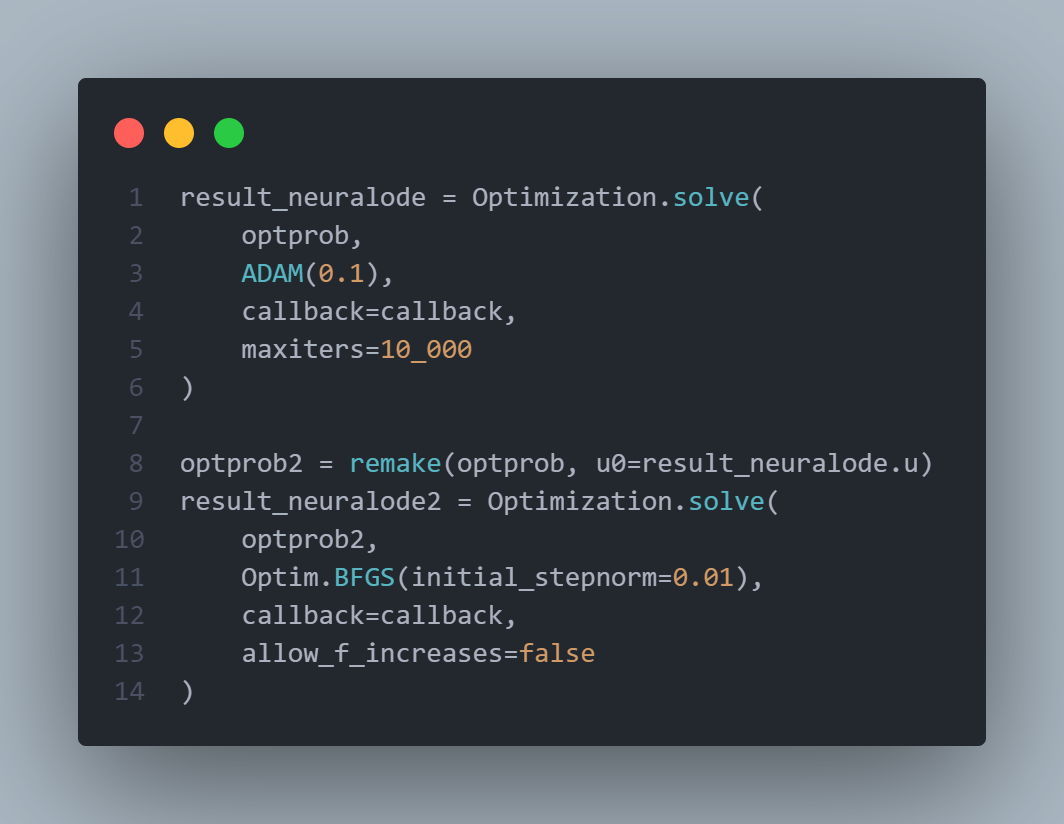
\includegraphics[width=\textwidth]{img/training.png}
	\captionof{figure}{Definizione delle funzioni di addestramento tramite due differenti ottimizzatori}
	\label{fig:training_function}
\end{minipage}

\subsubsection*{Predizione}
Viene utilizzato un approccio simile a quello denominato SINDy \cite{wiki:Sparse_identification_of_non-linear_dynamics}
per effettuare predizioni sul lungo termine fondendo un approccio \textbf{DataDriven} ad uno
\textbf{Domain Specific}.  

L'approccio \textbf{SINDy} ovvero Sparse Identification of Nonlinear Dynamics, e' un approccio algoritmico 
di tipo data-driven per ottenere sistemi dinamici partendo da un insieme di dati. In generale l'approccio e' 
quello di avere una serie di \emph{istantanee (snapshot)} del sistema e le loro corrispondenti derivate. A questo 
punto e' possibile effettuare un insieme di approcci di regressione come ad esempio \textbf{LASSO} \cite{wiki:Lasso_(statistics)}
per confrontare una molteplicita' di equazioni non lineari candidate con le derivate del sistema
per cercare di trovare le equazioni che governano l'intero sistema.

\begin{minipage}{\linewidth}
	\centering
	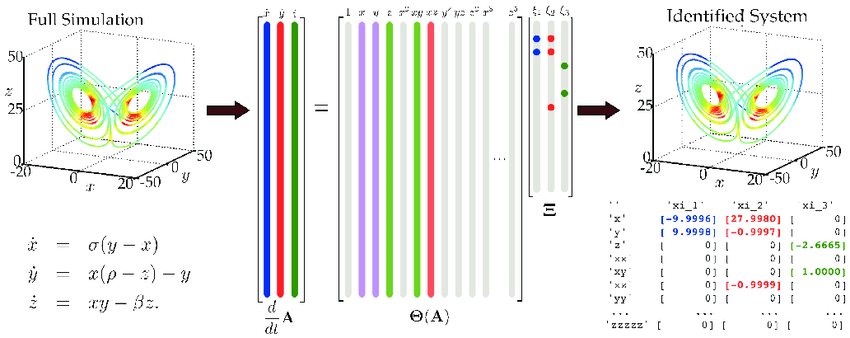
\includegraphics[width=\textwidth]{img/Schematic-of-the-sparse-identification-of-nonlinear-dynamics-SINDy-algorithm-25-as.png}
	\captionof{figure}{Esempio schematic del funzionamento di SINDy \cite{BruntonKutz+2021+307+344}}
	\label{fig:sindy}
\end{minipage}

Questa procedura si basa sull'assunzione che la maggior parte di sistemi fisici hanno una manciata
di equazioni dominanti che dettano l'evoluzione del sistema.

Seguendo quanto appena descritto, l'approccio si basa principalmente sull'utilizzo del modello 
appena creato e addestrato di Neural ODE, utilizzando due parti fondamentali di quest'ultimo

\begin{itemize}
	\item \textbf{$X$} che rappresenta il predittore del sistema.
	\item \textbf{$Y$} che rappresenta la derivate del sistema, o la predizione stessa.
\end{itemize}

Questi due elementi vengono successivamente inseriti all'interno di un algoritmo data-driven
per estrapolare le equazioni che governano il sistema, e successivamente vengono utilizzate 
queste equazioni in coppia con il vero sistema, da cui sono state ricavati i valori, 
che in questo caso e' conosciuto in quanto si sa che i valori sono generati da un sistema di tipo 
SEIR, per vedere se il sistema riesce a modellare i dati che non conosce, generealmente 
associati alla \textbf{FOI} o Force of Infection.

\begin{figure}[!hb]
	\centering
	\begin{subfigure}[b]{0.45\textwidth}
		\centering
		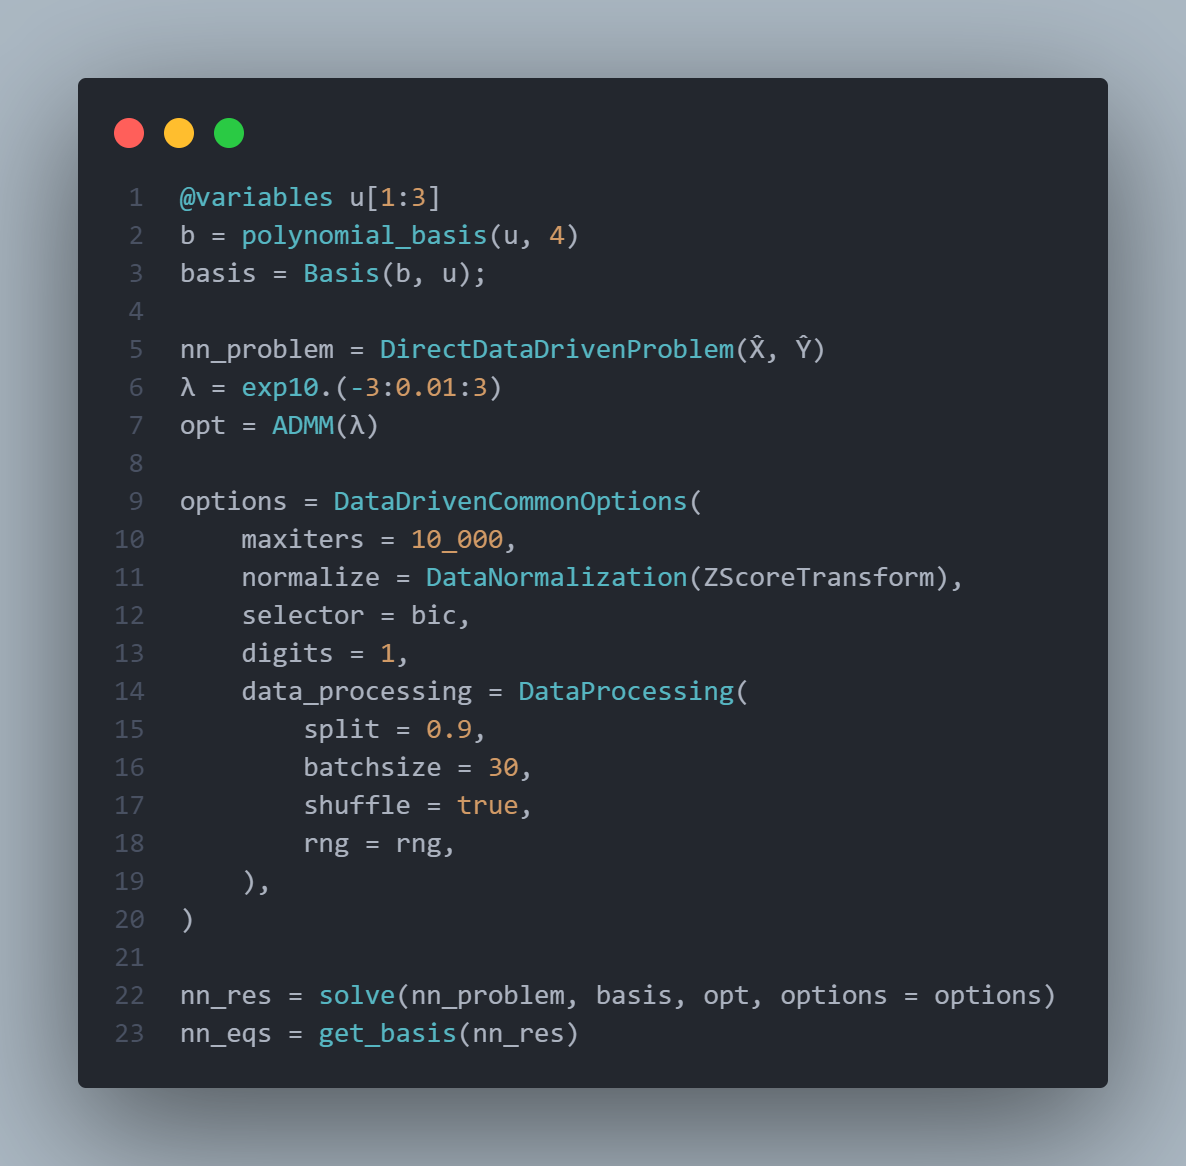
\includegraphics[width=\textwidth]{img/sindy_part_1.png}
		\caption{Codice relativo alla definizione del problema di tipo data-driven per SINDy}
		\label{fig:sindy_part_1}
	\end{subfigure}
	\hfill
	\begin{subfigure}[b]{0.45\textwidth}
		\centering
		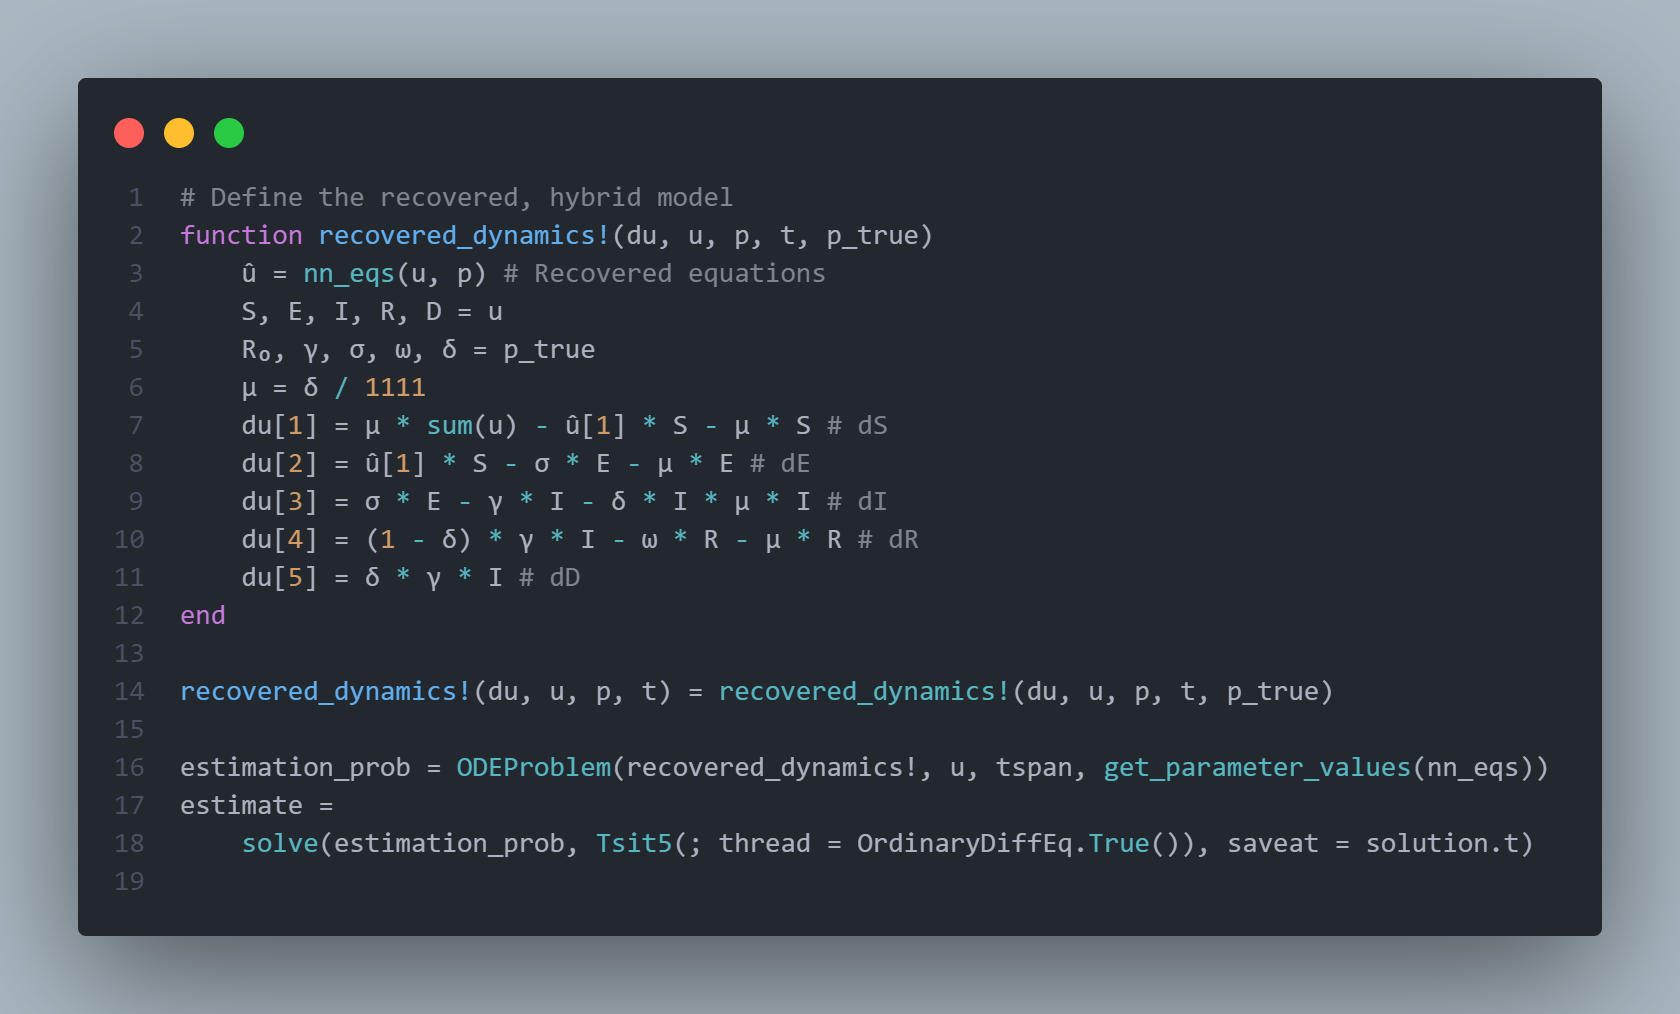
\includegraphics[width=\textwidth]{img/sindy_part_2.png}
		\caption{Codice relativo alla definizione del problema di tipo data-driven per SINDy}
		\label{fig:sindy_part_2}
	\end{subfigure}
\end{figure}

L'approccio e' simile a quello utilizzato per la Neural ODE precedentemente, ovvero si 
utilizza la liberia \textbf{Optim.jl} \cite{vaibhav_kumar_dixit_2023_7738525} per 
ottenere il risultato finale che si andra' ad utilizzare.

\subsubsection{Grafici}